\section{Atividade 8}

\subsection{Análise do Diagrama de Bode}

O método dos diagramas de Bode, introduzido por Hendrik Wade Bode, é uma ferramenta visual fundamental para analisar modelos de sistemas lineares. Ele é dividido em duas partes: diagrama de magnitude e diagrama de fase. Os diagramas de Bode são utilizados para verificar o desempenho do modelo e a estabilidade, além de auxiliar na implementação de sistemas de controle, facilitando o ajuste da sintonia de controladores.

\subsubsection{Código Scilab para obter o diagrama de Bode}

O código Scilab apresentado abaixo foi utilizado para gerar o diagrama de Bode do sistema massa-mola-amortecedor, permitindo a análise da resposta em frequência do sistema. Este código define os parâmetros do sistema, configura a função de transferência e plota o diagrama de Bode.

\begin{lstlisting}[language=Scilab, caption=Código Scilab para obter o diagrama de Bode]
    // Definicao dos parametros
    M = 10;
    C = 7;
    K = 5;

    // Funcao de transferencia
    num = 1;  // Numerador e um polinomio constante
    den = [M, C, K];  // Coeficientes do denominador
    den_poly = poly(den, 's', 'coeff');  // Criacao do polinomio do denominador

    // Sistema
    sys = syslin('c', num, den_poly);  // Correcao na criacao do sistema

    // Diagrama de Bode
    clf();
    bode(sys);
\end{lstlisting}

O código acima realiza as seguintes ações:
\begin{itemize}
    \item \textbf{Definição dos parâmetros:} Os valores de \( M \) (massa), \( C \) (coeficiente de amortecimento) e \( K \) (constante da mola) são definidos conforme especificado.
    \item \textbf{Configuração da função de transferência:} A função de transferência do sistema massa-mola-amortecedor é configurada utilizando os parâmetros definidos. O numerador da função de transferência é \(1\), enquanto o denominador é dado por \([M, C, K]\).
    \item \textbf{Criação do sistema:} O comando \texttt{syslin('c', num, den\_poly)} cria a representação do sistema linear contínuo com a função de transferência especificada.
    \item \textbf{Plot do Diagrama de Bode:} Os comandos \texttt{clf()} e \texttt{bode(sys)} limpam a figura atual e desenham o diagrama de Bode do sistema, respectivamente. O diagrama de Bode consiste em dois gráficos: magnitude (em dB) e fase (em graus) em função da frequência.
\end{itemize}
% Este código é fundamental para visualizar a resposta em frequência do sistema, permitindo uma análise detalhada das propriedades dinâmicas e da estabilidade do sistema massa-mola-amortecedor.

\subsubsection{Figura do Diagrama de Bode}

A Figura \ref{fig:Bode} apresenta o diagrama de Bode do sistema massa-mola-amortecedor com os parâmetros \(M = 10\), \(C = 7\), e \(K = 5\). O diagrama de Bode fornece informações valiosas sobre a resposta em frequência do sistema.

\begin{figure}[h]
    \centering
    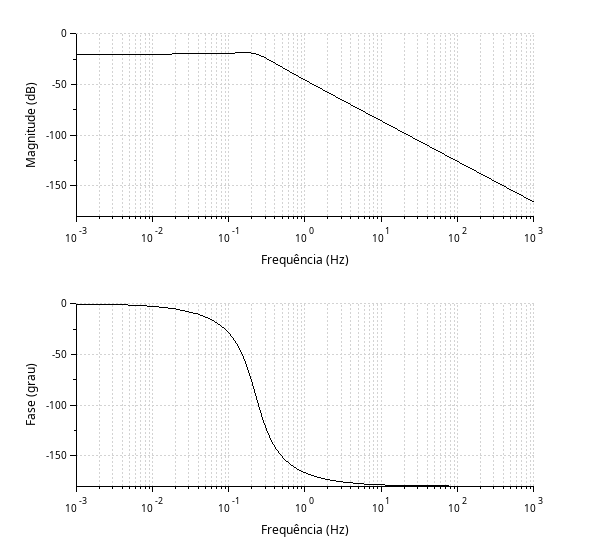
\includegraphics[width=0.8\textwidth]{atividades/8-atividade/assets/bode.png}
    \caption{Diagrama de Bode do sistema massa-mola-amortecedor.}
    \label{fig:Bode}
\end{figure}

\begin{itemize}
    \item \textbf{Gráfico de Magnitude:}
          O gráfico de magnitude, expresso em decibéis (dB), mostra que a magnitude começa em 0 dB para frequências muito baixas e depois decresce à medida que a frequência aumenta. Esse comportamento é característico de um filtro passa-baixa, útil para atenuar vibrações ou ruídos externos não desejados.. Não há pico de ressonância significativo, o que sugere que o sistema é bem amortecido.

          No gráfico, a magnitude cruza 0 dB em uma frequência de aproximadamente \(10^{-3} \, \text{Hz}\).

    \item \textbf{Gráfico de Fase:}
          O gráfico de fase, expresso em graus, mostra que a fase começa em 0 graus para frequências muito baixas, decresce gradualmente e se estabiliza próximo a -180 graus para frequências mais altas. A variação da fase indica a diferença de fase entre a entrada e a saída do sistema em diferentes frequências.

          A fase cruza -180 graus em uma frequência de aproximadamente \(10^1 \, \text{Hz}\), este comportamento indica a influência da massa, do amortecimento e da constante da mola na resposta do sistema.
    \item \textbf{Margens de Ganho e Fase:}
          \begin{itemize}
              \item \textbf{Margem de Ganho:} A margem de ganho representa o ganho adicional que o sistema pode suportar enquanto mantém a estabilidade em malha fechada. Este valor é medido no ponto em que a fase cruza -180 graus. No gráfico de magnitude, se a magnitude na frequência onde a fase é -180 graus estiver abaixo de 0 dB, a margem de ganho é positiva e o sistema é estável. No gráfico, observamos que a magnitude está bem abaixo de 0 dB na frequência onde a fase é -180 graus, indicando uma margem de ganho positiva.
              \item \textbf{Margem de Fase:} A margem de fase indica o quanto a fase do sistema pode ser atrasada sem que o sistema perca estabilidade em malha fechada. Este valor é medido na frequência onde a magnitude é 0 dB. No gráfico de fase, se a fase na frequência onde a magnitude é 0 dB estiver acima de -180 graus, a margem de fase é positiva e o sistema é estável. No gráfico, observamos que a fase está bem acima de -180 graus na frequência onde a magnitude é 0 dB, indicando uma margem de fase positiva.
          \end{itemize}
\end{itemize}

A análise dos diagramas de Bode gerados pelo código Scilab sugere que o sistema é estável, pois ambas as margens de ganho e fase são maiores que zero. Esta estabilidade implica que o sistema pode tolerar variações razoáveis no ganho e na fase sem perder a estabilidade. No entanto, é importante considerar que esta análise deve ser complementada com outras técnicas de análise de estabilidade para garantir uma avaliação completa.
